\chapter{Arquitectura de nodo basada en SoC}

En el capítulo anterior se han motivado el por qué de un cambio de arquitectura 
para el diseño de los nodos WR: aumento de la capacidad de cómputo, desarrollo 
de herramientas \textit{sw} más rápido y fácil, posibilidad de la inclusión de 
un SO, etc. Además gracias a las nuevas familias de SoC desarrolladas, ello no 
conlleva elevar en exceso el coste de fabricación del dispositivo. 
En este capítulo se discute la línea de trabajo e investigación actual para el 
desarrollo de nodos basados en SoC. Se explican los cambios necesarios para 
realizar una traslación del diseño actual del \gls{wrc2p} de la familia Artix-7 
(FPGA pura) a la familia Zynq-7000 (FPGA+ARM). Al final del capítulo se discute 
que línea se va a seguir en el futuro con motivo de aprovechar al máximo los 
recursos de la nueva plataforma basada en SoC y las posibles mejoras a la 
implementación inicial realizada para este tipo de plataforma.

\section{Características del diseño basado en SoC para Xilinx}

El diseño basado en SoC permite elevar el nivel de abstracción a la hora de 
definir los componentes que integrarán el sistema final. En concreto los SoC 
que incluyen FPGAs tienen la ventaja de ofrecer la flexibilidad de un sistema 
basado en FPGA (\textit{hardware} reconfigurable) con el rendimiento de los 
circuitos dedicados a tareas específicas, como un procesador de propósito 
general, un procesador digital de señales (DSP), interfaces de bus serie, 
controladores de memoria, y un largo etcétera. Cada fabricante suele ofrecer 
una serie de familias o gamas de productos en esta línea que se diferencian por 
los componentes físicos incluidos en el SoC y por las características de la 
FPGA. Para el caso que nos ocupa de desarrollo de un nodo WR, las 
características principales que debe poseer un SoC son:

\begin{itemize}
	\item Núcleo de lógica programable (FPGA). Obviamente toda la lógica 
	implementada en VHDL del núcleo WR se necesita implementar como 
	\textit{hardware} reconfigurable en una FPGA. Los requisitos de esta no son 
	demasiado exigentes ya que el diseño heredado ya estaba funcionando en una 
	FPGA de perfil bajo como la familia Spartan.
	
	\item Microprocesador de propósito general. Dadas las características 
	actuales de los nodos basados en FPGA con el LM32, cualquier core ARM de 
	los incorporados en los SoC de perfil bajo es suficiente para ofrecer la 
	capacidad de cómputo necesaria para este tipo de aplicaciones.
	
	\item Transceiver \incomment{rellenar}
	
	\item Interfaces DMA \incomment{rellenar}
	
	\incomment{pensar en más mierdas}
\end{itemize}

Con estos requisitos la familia Zynq-7000 encaja perfectamente tanto a la hora 
de cumplir los requisitos marcados anteriormente como en la de mantener un 
coste reducido. Los componentes principales de esta familia son los siguientes:

\begin{itemize}
	\item Microprocesador ARM Cortex-A9 de doble núcleo.
	\item Parte de lógica programable equivalente a un modelo Artix-7 (misma 
	familia que incopora el WR-LEN).
	\item Controlador de memoria con soporte para DDR3.
	\item Controlador \gls{dma} hacía módulos RAM externos.
	\item Ethernet MAC configurable a 10/100/1000 
\end{itemize}


\subsection{Arquitectura de la Familia Zynq-7000}
\incomment{arquitectura zynq-7, hablar un poco de los recursos y de como se 
organizan los componentes}

\subsection{Herramientas de desarrollo de Xilinx}
\incomment{hablar del nuevo modelo de trabajo basado en vivado y las cajitas}

\section{Migración y desarrollo de una arquitectura de nodo basada en SoC}

El llamado \textit{\acrlong{wr} Zynq Embedded Node} (WR-ZEN) es la primera 
plataforma que incorpora la nueva arquitectura para nodos basada en SoC. El 
desarrollo se ha realizado en colaboración entre la empresa Seven Solutions y 
el grupo de \textit{timing} de la UGR. \incomment{menciono esto para dejar 
claro que se habla de desarrollo de cosas que no he hecho aunque se menciona de 
forma ambigüa para dejar abierta la posibilidad de que se haya trabajado en 
ello}Dicho dispositivo será utilizado como 
elemento clave en el sistema de distribución de tiempo dentro del proyecto 
internacional SKA \cite{website:ska}. En concreto formará parte del llamado 
\textit{Signal and Data Transport (SaDT)} y se encargará de distribuir la señal 
de temporización a las antenas por medio de una señal \gls{pps}. El trabajo 
realizado en esta línea cuenta con varias publicaciones asociadas 
\cite{klyone16} \cite{klyone17}.

\subsection{Estructura del firmware de FPGA}

El diseño de la arquitectura añade un nivel de abstracción mayor en comparación 
al empleado en un nodo estándar como el \gls{spec} o el WR-LEN. La herramienta 
Vivado permite desarrollar la arquitectura mediante la inclusión de los módulos 
de alto nivel que representan las distintas unidades funcionales que componen 
el sistema. La Figura \ref*{fig:vivadozen} muestra el diagrama de bloques para 
la arquitectura del nodo ZEN. Los elementos principales a nivel de sistema son 
el \textit{Processing System}, el core-IP para la lógica WR (en la parte PL) y 
varios módulos para gestión de buses como los \textit{axi\_interconnect} y el 
\textit{axi\_quad\_spi}. Los elementos a este nivel se comunican mediante el 
bus 
AMBA o (en el caso del núcleo WR que se encuentra en la parte PL) necesitan un 
adaptador que haga de puente entre buses (\textit{axi\_interconnect}).

\begin{figure}
	\centering
	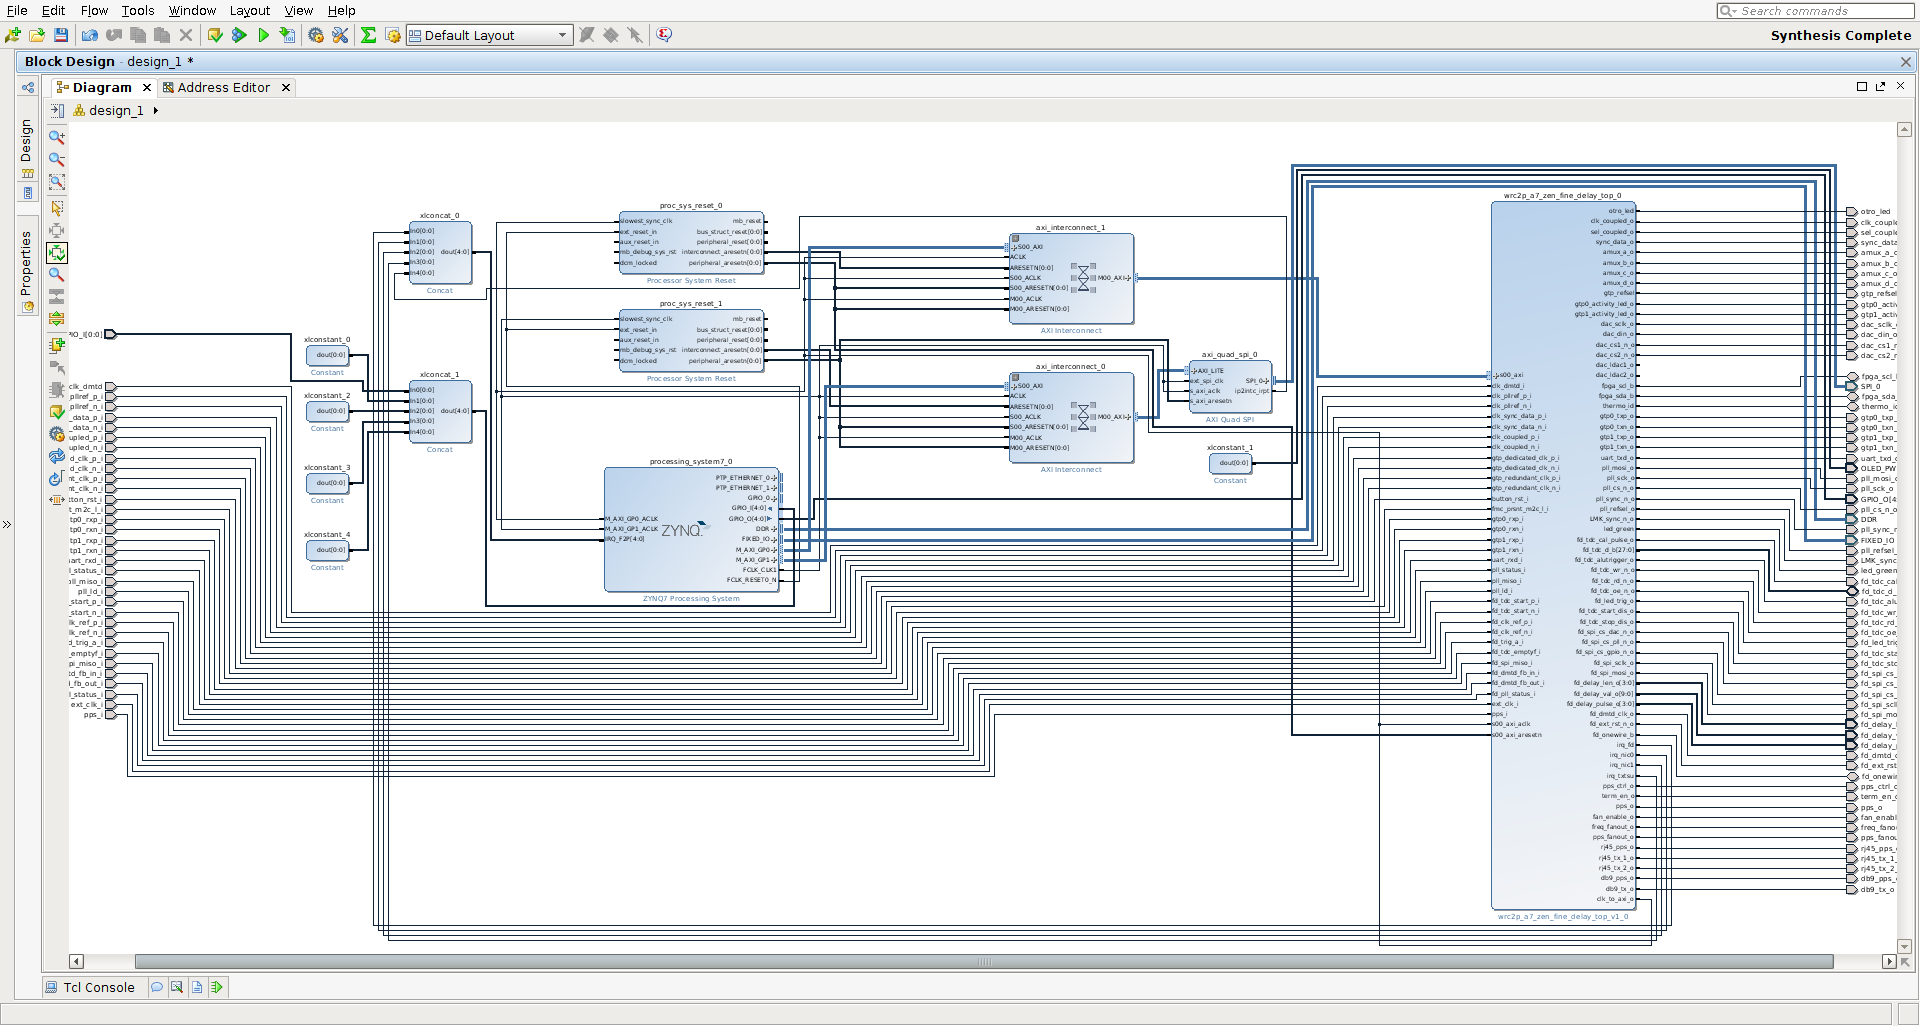
\includegraphics[width=0.8\linewidth]{imagenes/vivado_zen}
	\caption[Captura de Vivado con el diagrama de bloques de la arquitectura 
	del WR-ZEN]{Esta captura muestra el diagrama de bloques generado por Vivado 
	para mostrar los componentes de la arquitectura incluidos en el WR-ZEN.}
	\label{fig:vivadozen}
\end{figure}

El siguiente nivel de abstracción sería a nivel de core-IP donde se encuentra 
el núcleo WR correspondiente a la implementación \gls{wrc2p}. En una primera 
fase de adaptación de la antigua arquitectura de nodo basada en un diseño único 
de \gls{fpga} a la de SoC, se ha mantenido la estructura interna del núcleo WR, 
explicada en la sección ??, realizando cambios únicamente como adaptación a las 
peculiaridades de la familia Zynq-7000. Por ejemplo, se ha necesitado incluir 
un componente que convierta las transacciones del bus Wishbone utilizado en WR 
a las del bus AXI propio de la arquitectura Zynq. En líneas generales el diseño 
HDL \gls{wrc2p} utilizado en el WR-LEN presenta un alto nivel de compatibilidad 
con la nueva plataforma gracias a que la parte PL del modelo Zynq usado es una 
Artix-7. Por ello elementos como los envoltorios de los \textit{transceivers} 
que suele ser algo dependiente de la familia se han podido reutilizar sin 
mayores modificaciones.

\subsection{software}

El gran cambio con respecto al diseño anterior de nodo se encuentra actualmente 
en el ámbito del \textit{sw}. Los diseños anteriores para nodos implementaban 
todo el \textit{sw} de forma embebida, lo que suponía un coste elevado de 
desarrollo debido a la necesidad de un alto conocimiento de la plataforma 
subyacente y del resto de módulos que componen el código del sistema. Gracias a 
la potencia de cálculo extra del núcleo ARM se ha podido incluir un SO tipo 
Linux facilitando en gran medida el desarrollo de nuevas características o la 
inclusión de tecnologías ya existentes en el ecosistema Linux. Para lograr una 
correcta separación entre niveles de abstracción, se ha desarrollado una capa 
de abstracción \textit{hardware} (HAL) así como una serie de drivers que 
permiten acceder a la parte de lógica programable de forma homogénea por el 
\textit{sw} de usuario. Otro aspecto interesante es la mejora en la seguridad 
de los accesos al \textit{hw}, dado que existe una capa intermedia que arbitra 
los accesos evitando accesos indebidos o inconsistencias.

Dado que la complejidad de desarrollo ha aumentado bastante, ha sido necesario 
elaborar una serie de herramientas automáticas para la generación del kernel 
Linux y la compilación del resto de herramientas y \textit{sw} de forma 
parecida al sistema de compilación que existe para el \textit{sw} del 
\gls{wrs}. Dicho sistema automático de compilación se basa en una serie de 
\textit{scripts} que hacen de envoltorio para una herramienta muy conocida en 
este tipo de situaciones (Buildroot) de forma que se evita la necesidad de 
interacción por parte del usuario, facilitando así el despliegue del sistema 
para desarrolladores que necesiten trabajar sobre esta plataforma. El resultado 
es lo que se denomina \textit{root filesystem}, que no es más que una imagen 
del sistema de ficheros Linux para el arranque de la tarjeta.

\incomment{se puede hablar algo más de los módulos existentes (drivers)}

\incomment{esquema de las etapas de arranque}

Sin embargo, dicho \textit{root filesystem} no es lo único que se necesita para 
arrancar la tarjeta. Hay que recordar que se trata de un sistema embebido, por 
lo que se necesita un cargador de arranque inicial que se encargue de las 
tareas más básicas y de bajo nivel como inicializar los componentes \textit{hw} 
de la tarjeta. En la familia Zynq se utiliza un cargador de arranque llamado 
\textit{First Stage Bootloader} (FSBL) que ofrece un conjunto de operaciones 
muy restrigindas dado que no se pretende realizar ninguna tarea de alto nivel 
en esta etapa del arranque. Una de las tareas críticas realizadas por este 
componente de arranque es la inicialización y configuración de la parte PL. La 
última tarea que debe realizar es lanzar un cargador de segunda etapa que ya 
ofrece más flexibilidad a la hora de ser configurado para las necesidades 
específicas de la tarjeta. Además puede ser escogido por el desarrollador, 
contando con dos opciones principalmente que son Barebox y U-boot. Se ha optado 
por el segundo pues ofrece más funcionalidad que el primero y tiene una 
implementación más limpia y actualizada. Esta pieza de \textit{sw} permite 
realizar tareas más complejas de gestión de la tarjeta y termina 
descomprimiendo en memoria el \textit{root filesystem} y lanzando el kernel 
Linux, tras lo cual este toma posesión de la ejecución del procesador.

El desarrollo de todo este sistema ha supuesto un gran esfuerzo por parte de 
mucha gente tanto del grupo de la UGR como de la empresa Seven Solutions. Por 
ello se ha efectuado una primera fase donde se ha preparado el entorno, es 
decir, el SO, los drivers, HAL y demás herramientas de gestión, y se ha dejado 
para otra etapa el aprovechamiento real de la nueva arquitectura desde el punto 
de vista del núcleo de WR.

Por tanto, se mantiene el LM32 en la arquitectura WR. El código del PPSi y el 
resto de \textit{sw} embebido se sigue ejecutando en dicho 
\textit{soft-processor}. Aunque no se haya podido migrar dicho código al ARM, 
se ha conseguido descargar de muchas tareas secundarias de gestión al LM32 que 
si han sido llevadas a nivel de kernel o de usuario. La discusión de la línea 
de trabajo futura y de como organizar el núcleo WR para aprovechar esta nueva 
plataforma SoC se incluye en la sección \ref{sec:socfuturo}.

\section{El nodo WR-ZEN}

Al principio del capítulo ya se introducía una de las características más 
relevantes de esta nueva tarjeta WR llamada WR-ZEN: la incorporación de un SoC 
de la familia Zynq-7000. Gracias a la colaboración con Seven Solutions hemos 
podido disponer en el grupo de la universidad de este nuevo \textit{hw} para 
desarrollar toda la nueva línea de arquitectura y demás producción científica 
asociada a la mejora de WR.

\begin{figure}
	\centering
	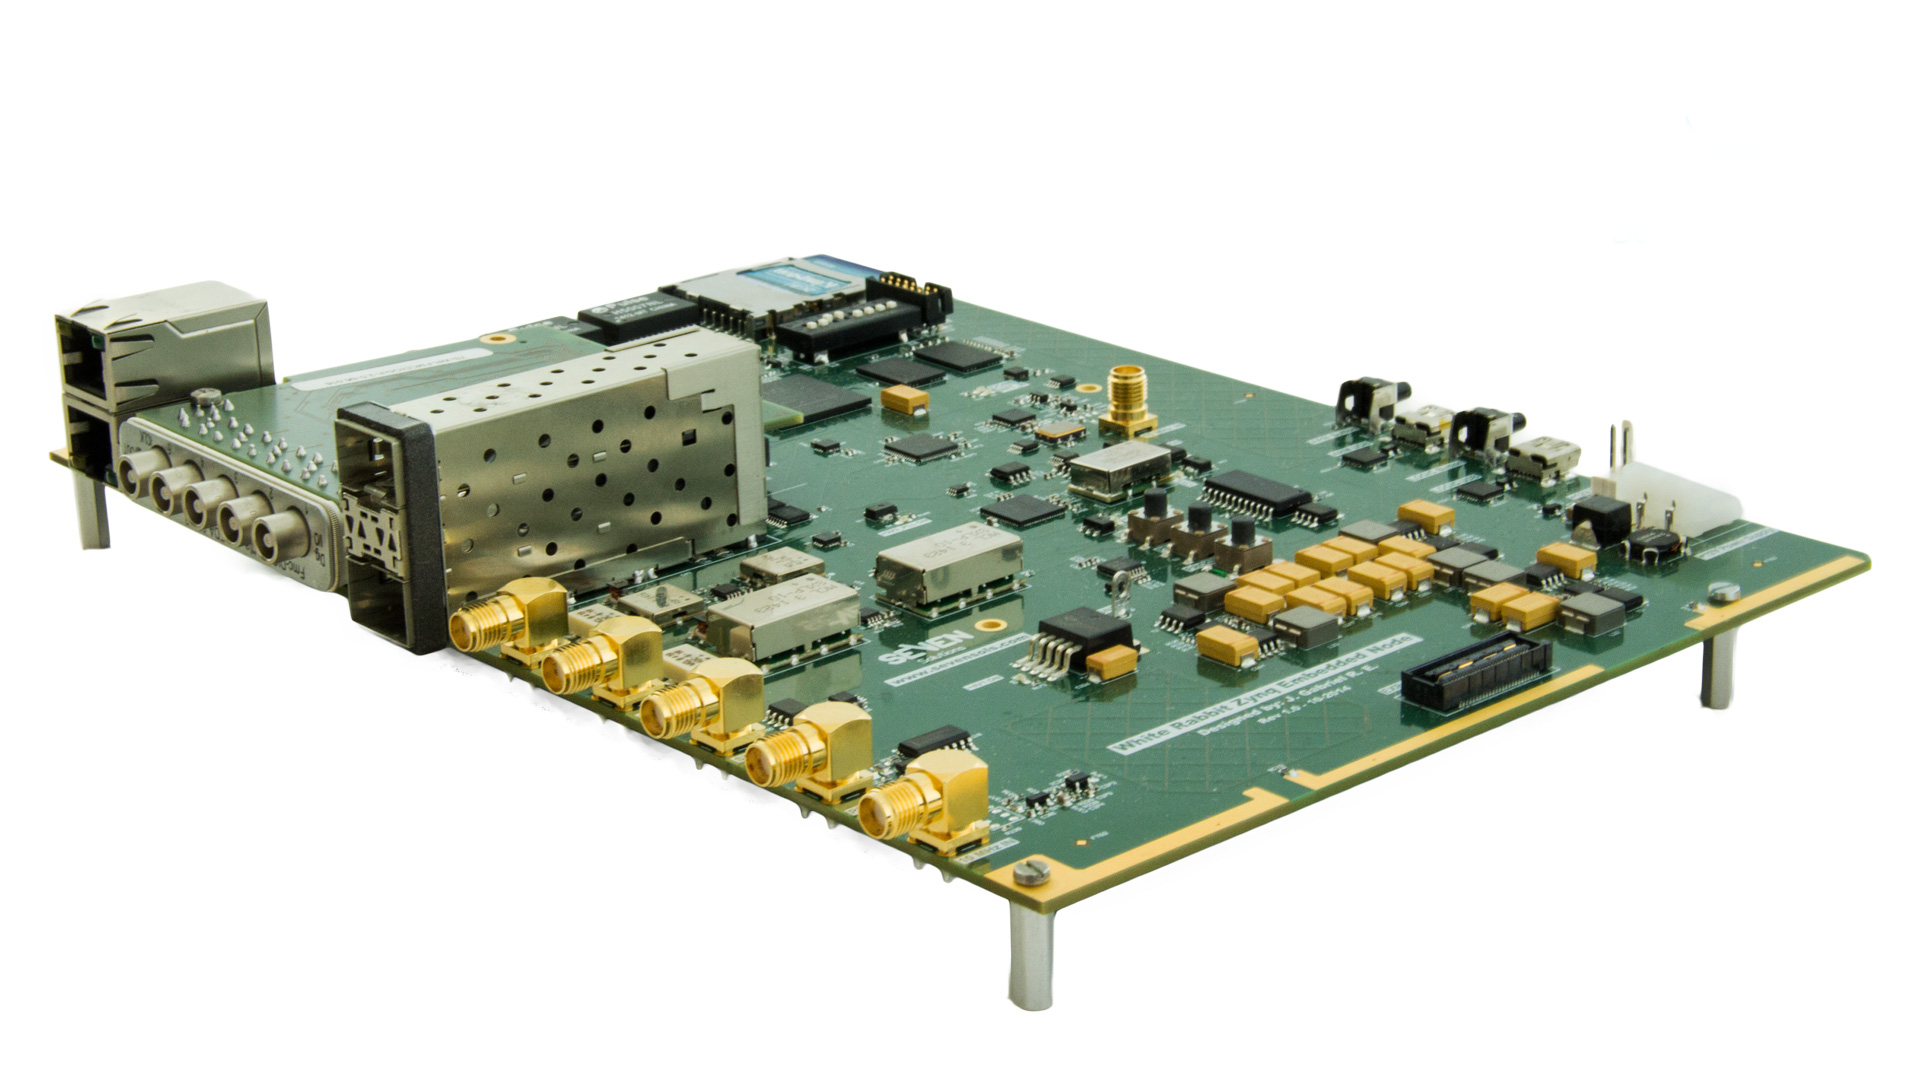
\includegraphics[width=0.7\linewidth]{imagenes/wrzen}
	\caption[Foto de la tarjeta WR-ZEN]{En la imagen de la PCB que forma el 
	nodo WR-ZEN se pueden observar los conectores de e/s SMA, los puertos 
	Ethernet para fibra y cobre, y el conector FMC que tiene una tarjeta de 
	adquisición conectada en la fotografía.}
	\label{fig:wrzen}
\end{figure}

En esta sección se pone el foco en los componentes \textit{hw} incluidos en 
este nuevo nodo ya que se han realizado varios cambios con respecto a la 
electrónica usual incluida en otros dispositivos WR como el \gls{wrs}, 
\gls{spec} o LEN.

\incomment{copiar aquí el párrafo de descripción del hw de la zen}

El nuevo esquema de reloj así como los distintos componentes nuevos que han 
sido introducidos me han permitido profundizar más en la electrónica de 
recuperación y generación de reloj para poder buscar formas de reducir el ruido 
del sistema desde la perspectiva más \textit{hw} del sistema. Dado que esto es 
algo bastante extenso he preferido dedicar un capítulo a parte 
(\ref{cap:reloj}) a todo lo relacionado 
con la electrónica de reloj, explicando como funciona el modelo actual, las 
mejoras al modelo que se investigan para el futuro y algunos resultados de 
pruebas experimentales que suponen una herramienta crucial a la hora de conocer 
este tipo de sistemas.

\section{Conclusiones y Trabajo futuro} \label{sec:socfuturo}

A lo largo de este capítulo se han descrito algunas de las ventajas que ofrece 
migrar la arquitectura del \textit{wrc} (o la variante de doble puerto) para 
nodos WR hacía una nueva plataforma basada en SoC: aumento de las prestaciones 
gracias al soporte \textit{hw} y una mayor flexibilidad de desarrollo gracias a 
la inclusión de un SO tipo Linux. Sin embargo, aún no se ha hecho uso realmente 
de todo el potencial que ofrece la nueva plataforma.

La estructura general presentada en \cite{Daniluk2012} y descrita de forma 
resumida en el diagrama de bloques de la Figura \ref{fig:wrpcinside} muestra 
una arquitectura de bus cuyo nexo de unión entre componentes es el bus Wishbone 
\textit{crossbar}. De esta forma la comunicación entre los diversos módulos y 
el procesador se realiza mediante accesos mapeados a memoria. Esta arquitectura 
deja de tener cierto sentido y se convierte en algo redundante si pensamos en 
la nueva plataforma basada en SoC. Si se realiza una migración de los modulos 
\textit{sw} que actualmente se ejecutan en el LM32, como el PPSi, al procesador 
ARM, es decir, a nivel de SO, ya sea en forma de drivers, o como programas de 
nivel de usuario, resulta que el \textit{sw} de control  necesita pasar primero 
por el puente AXI y luego por el bus Wishbone para llegar a los módulos en la 
parte PL. Por ello se propone una nueva arquitectura que realiza un 
aprovechamiento más eficiente de la nueva estructura de buses del SoC Zynq-7000 
y que se muestra en la Figura ?? \incomment{meter aquí un diagrama con los 
módulos colgando del AXI en vez del wb}. Para ello no habría que reimplementar 
la lógica de los módulos en HDL, si no que sería necesario añadir una capa que 
envuelva o reemplace la lógica de control pensada para el bus Wishbone por la 
del bus AXI. Para facilitar dicha labor se puede desarrollar una herramienta 
similar al \textit{wbgen2} que permita realizar una descripción de los 
registros de un componente en HDL y esta se encarge de generar de forma 
automática toda la lógica de control para la comunicación con el bus.

\incomment{imagen del nuevo esquema con el bus axi}

Sin embargo reemplazar por completo todos los componentes actuales no es algo 
trivial. Hay que tener en cuenta la lógica de control del módulo 
\textit{SoftPLL} que necesita cierto nivel de determinismo en su ejecución para 
realizar el cálculo del desfase y producir los valores consigna que se aplican 
para corregir la frecuencia de oscilación de los cristales disciplinados por WR 
en la tarjeta. Por tanto, se propone una primera fase donde se \textit{suban} 
de nivel el resto de módulos y se mantenga el bus wishbone para la lógica 
encargada del \textit{SoftPLL}. Esto sería una solución intermedia que se 
parece en parte a como funciona el LM32 en la arquitectura tipo \textit{switch}.

Para poder eliminar por completo el bus Wishbone sería necesaria una labor 
previa de investigación que analice y caracterice todo lo relacionado a la 
lógica de control del SoftPLL de manera que se pueda concluir si los requisitos 
temporales que tiene este algoritmo de control se pueden migrar a un sistema 
no-determinista como el Linux que corre ahora mismo a nivel de ARM. Otra 
posibilidad sería implementar la parte \textit{sw} del control del SoftPLL en 
HDL. ¿Por qué no se realizó desde un primer momento? Se podría pensar que es 
algo lógico pues la implementación en \textit{hw} asegura el determinismo y un 
nivel de prestaciones muy superior al alcanzable por la ejecución de un 
algoritmo \textit{sw} en un microprocesador. Sin embargo, hay que tener en 
cuenta que todo el diseño de WR es relativamente nuevo y por tanto, hay 
componentes que debido a su complejidad necesitan de una fase de implementación 
y testeo compleja. Según notas del autor de dicho código \incomment{tomasz 
tenía un documento que decía eso pero no lo encuentro por ningún lado 
ahora...}, esa fue una de las razones por las que parte del algoritmo de 
control se realizan en \textit{sw}. Dado que la tecnología ya cuenta con cierto 
grado de madurez, y que las metodologías de desarrollo para la generación de 
código en HDL han evolucionado mucho en los últimos años, se podría plantear 
una implementación en algún lenguage de descripción hardware de alto nivel como 
System-C, que permita la descripción del algoritmo a un nivel de abstracción 
mayor facilitando el proceso. Esto es algo que actualmente se está investigando 
en el grupo de sincronización de la UGR y que forma parte del núcleo de 
desarrollo de mi futura tésis.

Como conclusión de esta parte destacar la gran oportunidad, desde mi punto de 
vista, que supone el poder disponer de las soluciones en SoC que se están 
desarrollando en los últimos años, como es el caso de la familia Zynq-7000 de 
Xilinx. He podido comprobar de primera mano las restricciones que tiene la 
arquitectura tradicional para nodos basada únicamente en FPGA. Los recursos a 
nivel de \textit{sw} están muy limitados, tanto por el punto de vista del 
colapso del LM32 cuyo objetivo inicial era procesar una única interrupción y 
generar los valores de consigna para los osciladores disciplinados, y al que se 
le han ido añadiendo funcionalidades en forma de \textit{sw} embebido; como por 
la escasez de memoria fruto del uso de FPGAs de perfil bajo. Dado que un 
requisito de este tipo de dispositivos es mantener un coste bajo, no es una 
solución hacer uso de FPGAs con más recursos, lo cual pienso que no sería más 
que un parche pues se seguiría intentado aumentar el número de funcionalidades 
volviendo a colapsar los recursos. Además existe la posibilidad de incorporar 
algún procesador embebido distinto que ofrezca mayor rendimiento, por ejemplo 
el MicroBlaze de Xilinx. De nuevo opino que esto sería un parche y además 
necesitaría de un esfuerzo para adaptar el \textit{sw} a ese procesador. Por 
todo ello, creo que la solución SoC con un procesador físico ARM ofrece el 
mejor compromiso entre prestaciones y coste. Otro punto a su favor es la gran 
aceptación que tiene actualmente este tipo de microprocesadores, haciendo mucho 
más fácil todo lo relativo al desarrollo tanto a nivel de diseño de 
arquitectura como para los programas que se ejecutarán en el mismo.

Queda aún mucho trabajo por hacer para realizar un diseño que aproveche 
realmente las ventajas de la arquitectura ofrecida por la Zynq. Pero es 
importante ver la gran aceptación que está teniendo etre la comunidad 
científica el desarrollo del nodo WR-ZEN, que ya se ha incluido en proyectos de 
gran relevancia internacional como SKA, ya que esto favorece la publicación de 
nuevos artículos científicos que tengan interés en la comunidad relacionados 
con todo la investigación que se está haciendo en torno a este nuevo enfoque 
para nodos WR.

\incomment{ha quedado corto pero tampoco se donde me puedo estirar más}